\documentclass[10pt,a4paper]{article}
\usepackage{nexusS5}
\setnexusheader{Entrée en Quatrième — Stage de pré-rentrée}{Séance 5/5 — Ines KEFI}
\begin{document}
\nexuscover{SÉANCE 5 --- RÉINVESTIR, CONSOLIDER, PRÉPARER LA RENTRÉE}{Livret de travail}{Ines KEFI}{Transfert mixte et calibration de la confiance}{Entrée en Quatrième --- Mathématiques --- 1\,h\,15 de travail, puis 45 minutes d'évaluation dans un document séparé}
\begin{goalbox}
\textbf{Objectif personnel de cette séance.} Vérifier que les deux erreurs données avec une certitude maximale au diagnostic (ordre des relatifs, déplacement sur une droite graduée) ne réapparaissent plus, et que la transformation d'une fraction porte bien sur ses deux termes.
\par\medskip
\textbf{Ce livret couvre uniquement les 75 premières minutes.} L'évaluation finale est remise ensuite, dans un document distinct.
\end{goalbox}
\begin{methodbox}
\textbf{Le fil des cinq séances}
\begin{itemize}[leftmargin=13mm,labelsep=3mm,itemsep=1.5pt]
\item[\textbf{\color{Navy}S1}] Calculer avec du sens (relatifs, fractions) ;
\item[\textbf{\color{Navy}S2}] Mesurer une surface ou un contour (aires et périmètres) ;
\item[\textbf{\color{Navy}S3}] Donner du sens aux lettres (calcul littéral) ;
\item[\textbf{\color{Navy}S4}] Voir, raisonner, démontrer (géométrie) ;
\item[\textbf{\color{Navy}S5}] aujourd'hui : réactiver, consolider deux axes personnels, faire le pont vers la Quatrième, puis mesurer.
\end{itemize}
\end{methodbox}
\sectiontitle{Feuille de route des 75 minutes}
\rowcolors{2}{SoftBlue}{white}
\par\noindent\begin{tabularx}{\linewidth}{>{\bfseries}p{20mm} X X}
\rowcolor{Navy}\color{white}Temps & \color{white}Travail & \color{white}Preuve attendue \\
0--10 min & Remettre en activité sur les cinq domaines du stage et faire apparaître immédiatement les oublis. & Cinq réponses écrites et le contrôle utilisé. \\
10--35 min & Ordre des nombres relatifs et déplacements sur une droite graduée & Trois réussites autonomes sur l'axe prioritaire. \\
35--55 min & Fractions équivalentes et réduction au même dénominateur & Deux réussites autonomes sur le second axe. \\
55--70 min & De la Cinquième à la Quatrième : le signe d'un produit et la première équation & Une production reliant un acquis de Cinquième à un attendu de Quatrième. \\
70--75 min & Cadrage méthodologique, sans aucune information sur le contenu de l'évaluation. & Deux engagements écrits avant l'évaluation. \\
\end{tabularx}
\begin{graybox}\small\textbf{Règle de la séance.} J'écris ma réponse \emph{et} le contrôle qui la rend défendable. Une réponse sans contrôle reste une hypothèse. La ligne « Certitude » se remplit \emph{avant} toute vérification.\end{graybox}
\par\vspace{2mm}
\phasehead{Phase 1 --- Réactivation}{0--10 min}{Remettre en activité sur les cinq domaines du stage et faire apparaître immédiatement les oublis.}
Sept minutes seules, sans carte de rappel, puis trois minutes de mise en commun. Écrire la réponse \emph{et} le contrôle utilisé.
\begin{enumerate}
\item Calculer $(-9) + 4 - (-6)$.
\shortlines{2}
\item Calculer $\dfrac{7}{10} - \dfrac{2}{5}$ en transformant entièrement la seconde fraction.
\shortlines{2}
\item Réduire $6x - 5 + 2x + 9$, puis contrôler pour $x = 1$.
\shortlines{2}
\item Deux angles d'un triangle mesurent $43^\circ$ et $68^\circ$. Calculer le troisième en citant la propriété.
\shortlines{2}
\item Un rectangle mesure 11 cm sur 6 cm. Donner son aire et son périmètre, unités comprises.
\shortlines{2}
\end{enumerate}
\certline
\aideline
\needspace{62mm}\par\vspace{3mm}
\phasehead{Phase 2 --- Consolidation, axe prioritaire}{10--35 min}{Ordre des nombres relatifs et déplacements sur une droite graduée}
\begin{methodbox}
\textbf{Trois repères.} Ranger dans l'ordre \textbf{croissant}, c'est lire la droite graduée de la \textbf{gauche vers la droite}.
Se déplacer vers la droite, c'est \textbf{ajouter} ; vers la gauche, c'est \textbf{soustraire}.
Entre deux nombres négatifs, le plus grand est celui qui est le plus \textbf{proche de zéro}.
\end{methodbox}
\begin{center}
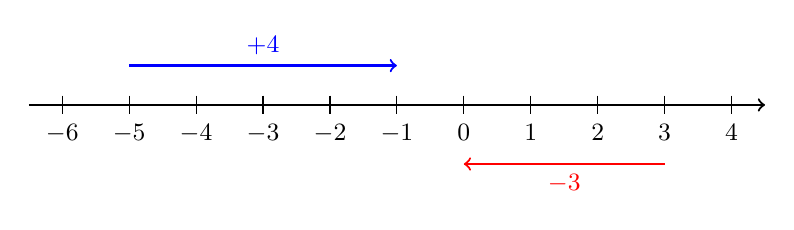
\begin{tikzpicture}[x=0.85cm]
\draw[->,thick] (-6.5,0) -- (4.5,0);
\foreach \x in {-6,-5,-4,-3,-2,-1,0,1,2,3,4}{\draw (\x,0.12) -- (\x,-0.12) node[below]{\small $\x$};}
\draw[->,Blue,thick] (-5,0.5) -- (-1,0.5) node[midway,above]{\small $+4$};
\draw[->,Red,thick] (3,-0.75) -- (0,-0.75) node[midway,below]{\small $-3$};
\end{tikzpicture}
\end{center}
\begin{graybox}
\textbf{Exemple guidé.} Ranger dans l'ordre croissant : $-8$ ; $3$ ; $-2$ ; $0$ ; $-11$.
\begin{enumerate}
\item Placer mentalement chaque nombre sur la droite.
\item Lire de gauche à droite : $-11$ ; $-8$ ; $-2$ ; $0$ ; $3$.
\item Contrôler : les négatifs se rangent « à l'envers » des nombres positifs correspondants ($11 > 8 > 2$ devient $-11 < -8 < -2$).
\end{enumerate}
\end{graybox}
\subsectiontitle{À toi}
\begin{enumerate}
\needspace{18mm}
\item Ranger dans l'ordre croissant : $-6$ ; $1$ ; $-13$ ; $0$ ; $-4$.
\worklines{2}
\needspace{18mm}
\item Ranger dans l'ordre décroissant : $-9$ ; $5$ ; $-2$ ; $7$.
\worklines{2}
\needspace{18mm}
\item Un point d'abscisse $-13$ se déplace de $17$ unités vers la droite. Donner son abscisse finale.
\worklines{2}
\needspace{18mm}
\item Un point d'abscisse $6$ se déplace de $11$ unités vers la gauche. Donner son abscisse finale.
\worklines{2}
\needspace{18mm}
\item Comparer $-17$ et $-8$, puis justifier la réponse par une phrase et non par une règle apprise.
\worklines{3}
\needspace{18mm}
\item Un élève range $-3$ ; $-7$ ; $-10$ en écrivant « $-3 < -7 < -10$ ». Expliquer l'erreur, corriger, puis indiquer le contrôle qui l'aurait évitée.
\worklines{4}
\end{enumerate}
\begin{successbox}\textbf{Critère de réussite de cette phase :} quatre classements ou déplacements corrects consécutifs, chacun justifié oralement par la position sur la droite.\end{successbox}
\certline
\needspace{62mm}\par\vspace{3mm}
\phasehead{Phase 3 --- Consolidation, second axe}{35--55 min}{Fractions équivalentes et réduction au même dénominateur}
\begin{methodbox}
\textbf{Transformer une fraction, c'est transformer ses deux termes.} Multiplier le numérateur \emph{et}
le dénominateur par un même nombre non nul ne change pas la valeur de la fraction :
$\dfrac{a}{b}=\dfrac{a\times k}{b\times k}$. Si un seul terme est modifié, la fraction change de valeur.
\textbf{Contrôle :} une différence de deux fractions positives doit être plus petite que la première.
\end{methodbox}
\subsectiontitle{À toi}
\begin{enumerate}
\needspace{18mm}
\item Compléter $\dfrac{3}{4}=\dfrac{\ldots}{20}$ et écrire le facteur utilisé.
\worklines{2}
\needspace{18mm}
\item Calculer $\dfrac{5}{9}-\dfrac{1}{3}$.
\worklines{2}
\needspace{18mm}
\item Calculer $\dfrac{3}{4}+\dfrac{5}{12}$.
\worklines{2}
\needspace{18mm}
\item Calculer $\dfrac{7}{8}-\dfrac{3}{16}$.
\worklines{2}
\end{enumerate}
\begin{successbox}\textbf{Critère de réussite de cette phase :} quatre soustractions ou additions consécutives exactes, la transformation complète de chaque fraction étant écrite.\end{successbox}
\certline
\needspace{62mm}\par\vspace{3mm}
\phasehead{Phase 4 --- Réinvestissement}{55--70 min}{Découverte guidée : construire, à partir d'acquis de Cinquième, deux notions nouvelles de Quatrième — le signe d'un produit de relatifs et l'équation du premier degré.}

\begin{methodbox}
\textbf{Ce qui change en Quatrième.} L'addition et la soustraction des relatifs sont supposées acquises :
elles ont été travaillées en séance 1. La Quatrième y ajoute le \textbf{produit} et le \textbf{quotient} de
relatifs, puis utilise les expressions littérales pour écrire et résoudre des \textbf{équations}.
\par\smallskip
Ces deux notions sont \textbf{nouvelles}. Les blocs ci-dessous ne sont donc pas un réemploi : ce sont deux
\textbf{découvertes guidées}. Chacune part d'un acquis de Cinquième — le sens des signes, l'écriture d'une
expression littérale — pour construire la règle nouvelle pas à pas.
\end{methodbox}
\begin{warningbox}\small
\textbf{Cette phase introduit des notions de l'année à venir.} Ce que tu produis ici ne sera donc
\emph{pas} comparé à ton positionnement de début de stage : il ne s'agit pas de mesurer un progrès,
mais de préparer les premières séances de septembre.
\end{warningbox}


\subsectiontitle{A. Le signe d'un produit — 6 min}
Compléter le tableau, puis écrire la règle en une phrase.
\par\noindent\begin{tabularx}{\linewidth}{>{\bfseries}p{30mm} X >{\bfseries}p{30mm} X}
\toprule
Produit & Résultat & Produit & Résultat \\
\midrule
$3 \times (-4)$ & & $(-3)\times(-4)$ & \\
$(-5)\times 2$ & & $(-5)\times(-2)$ & \\
\bottomrule
\end{tabularx}
\par\vspace{1mm}
Ma règle : \rule{125mm}{0.32pt}
\par\vspace{1mm}
Contrôle demandé : donner un produit de deux nombres dont le résultat est $-12$, puis un autre, différent.
\shortlines{1}

\subsectiontitle{B. Écrire puis résoudre une équation — 9 min}
Une salle est louée $35$ TND, auxquels s'ajoutent $4$ TND par participant.
\begin{enumerate}
\item Écrire l'expression $C(n)$ du coût pour $n$ participants. \rule{60mm}{0.32pt}
\item Calculer $C(12)$ en montrant la substitution.
\shortlines{1}
\item La facture s'élève à $99$ TND. Écrire l'équation correspondante, puis la résoudre en écrivant chaque étape.
\worklines{3}
\item Contrôler la solution trouvée en la remplaçant dans $C(n)$.
\shortlines{1}
\end{enumerate}

\begin{successbox}
\textbf{Preuve attendue :} l'expression est écrite avant tout calcul ; la solution de l'équation est
contrôlée par substitution et non par une simple relecture.
\end{successbox}

\needspace{62mm}\par\vspace{3mm}
\phasehead{Phase 5 --- Avant l'évaluation}{70--75 min}{Cadrage méthodologique. Aucun contenu de l'évaluation n'est annoncé.}

\begin{methodbox}
\textbf{Cinq règles, et rien d'autre.} Ce cadrage ne porte sur aucun contenu de l'évaluation.
\begin{enumerate}
\item \textbf{Gérer le temps.} Trois parties : environ 10 min, 20 min et 15 min. Un regard sur l'horloge à la fin de chaque partie suffit.
\item \textbf{Justifier.} Écrire la relation, la propriété ou la règle avant le calcul. Un résultat seul ne montre pas ce que tu sais.
\item \textbf{Contrôler.} Avant de passer à la suite : ordre de grandeur, substitution, unité, ou vérification par une seconde voie.
\item \textbf{Lire jusqu'au bout.} Souligner la question réellement posée et les données effectivement fournies.
\item \textbf{Passer et revenir.} Une question laissée de côté puis reprise vaut mieux qu'une réponse écrite au hasard.
\end{enumerate}
\end{methodbox}

\begin{graybox}
\textbf{La certitude.} Elle est demandée à trois moments seulement, comme au test de positionnement de début de stage :
\conf\ . Elle n'entre pas dans la note. Elle sert à distinguer ce que tu sais de ce que tu crois savoir.
\end{graybox}

\subsectiontitle{Mon engagement d'avant-évaluation}
\par\vspace{1mm}
\noindent\textbf{Le contrôle que j'écrirai systématiquement :}\ \rule{\dimexpr\linewidth-76mm\relax}{0.32pt}
\par\vspace{3mm}
\noindent\textbf{La question que je traiterai en dernier :}\ \rule{\dimexpr\linewidth-68mm\relax}{0.32pt}
\par\vspace{1mm}

\begin{warningbox}\textbf{Fin du livret de travail.} L'évaluation finale est un document séparé, remis par l'enseignant à l'issue de ces 75 minutes.\end{warningbox}
\end{document}
